\chapter{Presentación de Resultados}
	\section{Introducción} 
	
	Este capítulo presenta los resultados obtenidos durante la implementación de cada uno de los prototipos planteados en el Capítulo
	~\ref{chap:disenoeimpl} y durante la ejección de los casos de prueba correspondientes. 
	
	Para la ejecución de todas las pruebas se utilizó la placa desarrollo S3ADSP1800A del fabricante Xilinx que cumple con los requerimientos detallados
	en la Tabla ~\ref{tab:requsr1} y se encontraba dentro de las alternativas disponibles al momento del desarrollo de este trabajo. Aún cumpliendo con
	los requerimientos especificados, la placa de desarrollo no cuenta con un completo soporte de periféricos on board ni con amplia documentación de
	apoyo respecto de la materia. Se presentaron grandes dificultades en el acceso a la memoria SPI FLASH S33 de Intel la cual se encuentra soportada por
	herramientas \textit{oficiales} que únicamente corren bajo Windows. Alternativamente existe una versión de la placa de desarrollo S3ADSP1800A,
	disponible también en el laboratorio del CUDAR, que se encuentra equipada con una memoria FLASH SPI Numonyx M25P64 que puede ser accedida mediante
	herramientas de programación como XC3SPROG y UrJTAG alojando finalmente los programas necesarios para el arranque del sistema.
	
	Las pruebas realizadas con el sistema operativo de tiempo real ecOS proveyeron información útil para el desarrollo de sistemas embebidos de tiempo
	real. Se analizaron inicialmente las capacidades y limitaciones en la ejecución de hilos. Aunque estas pruebas tan solo verifican la utilización de
	una parte las capacidades, el sistema operativo ecOS posee mayor funcionalidad que no fue probada en este trabajo y presenta capacidades comparables
	a implementaciones como lo son FreeRTOS y su implentación comercial eCosPro.
	
	La capacidad, por defecto, del Kernel de Linux de ser compilado para arquitecturas OpenRISC posibilitó tener un entorno de ejecución de amplia
	funcionalidad y gran utilización en el ámbito de desarrollo de Sistemas Embebidos.  
	
	\section{Estudio de capacidades del proyecto MinSoC}
	El proyecto MinSoC se encuentra enfocado a su utilización en sistemas embebidos de capacidades ajustadas sintetizables en una gran cantidad de FPGA
	de diversos desarrolladores. La facilidad de adaptación del proyecto para ser portado a otras arquitecturas reconfigurables le confiere gran
	versatilidad ampliando notablemente su gama de aplicación.
	Durante el desarrollo de las pruebas se prentendió esteblecer los límites de aplicación del proyecto que establezcan referencias sólidas para una
	futura elección del proyecto en aplicaciones reales.

		\subsection{Resultados de la ejecución del multiplicador de matrices binarias}
		
\begin{figure}[h!]
 	\begin{center}
  	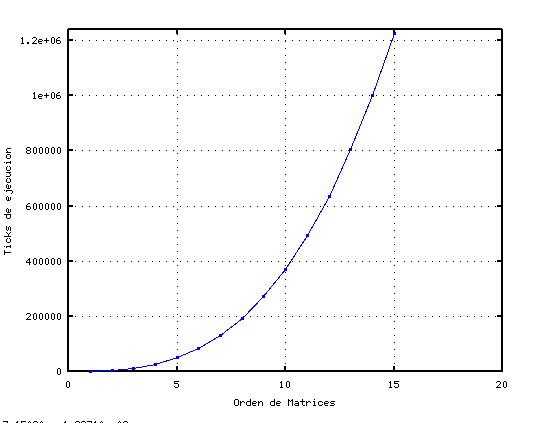
\includegraphics[width=0.6\textwidth,keepaspectratio=true]{./images/matrices}
  	\caption{Multiplicación de Matrices Binarias}
  	%\label{fig:mulmat}
 	\end{center}
	\end{figure}

\newpage
	\section{Estudio de capacidades del proyecto ORPSoC}

		
			\subsection{Condiciones del entorno de ejecución}
		En la siguente tabla ~\ref{tab:conbench} se muestran las condiciones durante los benchmarks

\begin{table}[!h]
\begin{tabular}{ |p{5cm} |p{10cm}| }    
\hline
\multicolumn{2}{|>{\columncolor[gray]{.8}}c}{Condiciónes de entorno de prueba|}\\
		\hline
		Placa de desarrollo & S3ADSP1800A  \\
		\hline 
		FPGA & Xilinx Spartan-3 XC3SD1800A \\ 
		\hline 
		Reloj del procesador & 25 MHz\\ 
		\hline
		Caché de instrucciones  & 8 KB \\ 
		\hline
		Caché de datos	  & 8 KB\\ 
		\hline	
		MMU & Sí \\	
		\hline
		Multiplicador hardware & Sí \\		
		\hline	
		División hardware & Sí \\		
		\hline	
\end{tabular}
%\end{center}
%\caption{Listado de requerimientos de usuario - Licencias}
\label{tab:conbench}
\end{table}

				\subsection{Resultados de la ejecución del Benchmark CoreMark}
		
Esto le da un valor de CoreMark 41288895/25MHz = 1.65/MHz. Se trato de de mejorar este valor mediante la adición de algunas opciones del compilador.

Aquí están los resultados de tratar de optimizar la fase de compilación. Al ser compilado con el nivel de optimización -O2 se observaron los resultados mostrados en el bloque ~\ref{lst:salidas} 

\begin{lstlisting}[frame=single,caption={Optimización nivel -O2},label={lst:salidas},breaklines]
Iterations/Sec   : 39.292731
Iterations       : 600
Compiler version : GCC4.5.1-or32-1.0rc4
Compiler flags   : -O2  -mboard=s3adsp1800a -FUNROLL-LOOPS -DVALIDATION_RUN=1  
Memory location  : STACK
seedcrc          : 0x18f2
[0]crclist       : 0xe3c1
[0]crcmatrix     : 0x0747
[0]crcstate      : 0x8d84
[0]crcfinal      : 0xb8a0
\end{lstlisting}

\begin{lstlisting}[frame=single,caption={Optimización nivel -O2},label={lst:salidas},breaklines]
2K validation run parameters for coremark.
CoreMark Size    : 666
Total ticks      : 1528
Total time (secs): 15.280000
Iterations/Sec   : 39.267016
Iterations       : 600
Compiler version : GCC4.5.1-or32-1.0rc4
Compiler flags   : -O2  -mboard=s3adsp1800a -MSOFT-FLOAT -DVALIDATION_RUN=1  
Memory location  : STACK
seedcrc          : 0x18f2
[0]crclist       : 0xe3c1
[0]crcmatrix     : 0x0747
[0]crcstate      : 0x8d84
[0]crcfinal      : 0xb8a0
\end{lstlisting}

\begin{lstlisting}[frame=single,caption={Optimización nivel -O2},label={lst:salidas},breaklines]
2K validation run parameters for coremark.
CoreMark Size    : 666
Total ticks      : 1528
Total time (secs): 15.280000
Iterations/Sec   : 39.267016
Iterations       : 600
Compiler version : GCC4.5.1-or32-1.0rc4
Compiler flags   : -O2  -mboard=s3adsp1800a -FUNROLL-ALL-LOOPS -DVALIDATION_RUN=1  
Memory location  : STACK
seedcrc          : 0x18f2
[0]crclist       : 0xe3c1
[0]crcmatrix     : 0x0747
[0]crcstate      : 0x8d84
[0]crcfinal      : 0xb8a0
\end{lstlisting}

\begin{lstlisting}[frame=single,caption={Optimización nivel -O2},label={lst:salidas},breaklines]
2K validation run parameters for coremark.
CoreMark Size    : 666
Total ticks      : 1527
Total time (secs): 15.270000
Iterations/Sec   : 39.292731
Iterations       : 600
Compiler version : GCC4.5.1-or32-1.0rc4
Compiler flags   : -O2  -mboard=s3adsp1800a -FGCSE-SM -DVALIDATION_RUN=1  
Memory location  : STACK
seedcrc          : 0x18f2
[0]crclist       : 0xe3c1
[0]crcmatrix     : 0x0747
[0]crcstate      : 0x8d84
[0]crcfinal      : 0xb8a0
\end{lstlisting}

\begin{lstlisting}[frame=single,caption={Optimización nivel -O3},label={lst:salidas},breaklines]
2K validation run parameters for coremark.
CoreMark Size    : 666
Total ticks      : 1654
Total time (secs): 16.540000
Iterations/Sec   : 36.275695
Iterations       : 600
Compiler version : GCC4.5.1-or32-1.0rc4
Compiler flags   : -O3  -mboard=s3adsp1800a -DVALIDATION_RUN=1  
Memory location  : STACK
seedcrc          : 0x18f2
[0]crclist       : 0xe3c1
[0]crcmatrix     : 0x0747
[0]crcstate      : 0x8d84
[0]crcfinal      : 0xb8a0
\end{lstlisting}
\begin{lstlisting}[frame=single,caption={Optimización nivel -O3},label={lst:salidas},breaklines]
2K validation run parameters for coremark.
CoreMark Size    : 666
Total ticks      : 1654
Total time (secs): 16.540000
Iterations/Sec   : 36.275695
Iterations       : 600
Compiler version : GCC4.5.1-or32-1.0rc4
Compiler flags   : -O3  -mboard=s3adsp1800a -MHARD-DIV -MHARD-MULT -DVALIDATION_RUN=1  
Memory location  : STACK
seedcrc          : 0x18f2
[0]crclist       : 0xe3c1
[0]crcmatrix     : 0x0747
[0]crcstate      : 0x8d84
[0]crcfinal      : 0xb8a0
\end{lstlisting}
\begin{lstlisting}[frame=single,caption={Optimización nivel -O3},label={lst:salidas},breaklines]
2K validation run parameters for coremark.
CoreMark Size    : 666
Total ticks      : 1654
Total time (secs): 16.540000
Iterations/Sec   : 36.275695
Iterations       : 600
Compiler version : GCC4.5.1-or32-1.0rc4
Compiler flags   : -O3  -mboard=s3adsp1800a -FUNROLL-LOOPS -DVALIDATION_RUN=1  
Memory location  : STACK
seedcrc          : 0x18f2
[0]crclist       : 0xe3c1
[0]crcmatrix     : 0x0747
[0]crcstate      : 0x8d84
[0]crcfinal      : 0xb8a0
\end{lstlisting}
\begin{lstlisting}[frame=single,caption={Optimización nivel -O3},label={lst:salidas},breaklines]
2K validation run parameters for coremark.
CoreMark Size    : 666
Total ticks      : 1655
Total time (secs): 16.550000
Iterations/Sec   : 36.253776
Iterations       : 600
Compiler version : GCC4.5.1-or32-1.0rc4
Compiler flags   : -O3  -mboard=s3adsp1800a -FUNROLL-LOOPS -DVALIDATION_RUN=1  
Memory location  : STACK
seedcrc          : 0x18f2
[0]crclist       : 0xe3c1
[0]crcmatrix     : 0x0747
[0]crcstate      : 0x8d84
[0]crcfinal      : 0xb8a0
\end{lstlisting}
\begin{lstlisting}[frame=single,caption={Optimización nivel -O3},label={lst:salidas},breaklines]
2K validation run parameters for coremark.
CoreMark Size    : 666
Total ticks      : 1654
Total time (secs): 16.540000
Iterations/Sec   : 36.275695
Iterations       : 600
Compiler version : GCC4.5.1-or32-1.0rc4
Compiler flags   : -O3  -mboard=s3adsp1800a -FGCSE-SM -DVALIDATION_RUN=1  
Memory location  : STACK
seedcrc          : 0x18f2
[0]crclist       : 0xe3c1
[0]crcmatrix     : 0x0747
[0]crcstate      : 0x8d84
[0]crcfinal      : 0xb8a0
\end{lstlisting}
\begin{lstlisting}[frame=single,caption={Optimización nivel -O3},label={lst:salidas},breaklines]
2K validation run parameters for coremark.
CoreMark Size    : 666
Total ticks      : 1655
Total time (secs): 16.550000
Iterations/Sec   : 36.253776
Iterations       : 600
Compiler version : GCC4.5.1-or32-1.0rc4
Compiler flags   : -O3  -mboard=s3adsp1800a -MSOFT-FLOAT -DVALIDATION_RUN=1  
Memory location  : STACK
seedcrc          : 0x18f2
[0]crclist       : 0xe3c1
[0]crcmatrix     : 0x0747
[0]crcstate      : 0x8d84
[0]crcfinal      : 0xb8a0
\end{lstlisting}
\begin{lstlisting}[frame=single,caption={Optimización nivel -O3},label={lst:salidas},breaklines]
2K validation run parameters for coremark.
CoreMark Size    : 666
Total ticks      : 1654
Total time (secs): 16.540000
Iterations/Sec   : 36.275695
Iterations       : 600
Compiler version : GCC4.5.1-or32-1.0rc4
Compiler flags   : -O3  -mboard=s3adsp1800a -FUNROLL-ALL-LOOPS -DVALIDATION_RUN=1  
Memory location  : STACK
seedcrc          : 0x18f2
[0]crclist       : 0xe3c1
[0]crcmatrix     : 0x0747
[0]crcstate      : 0x8d84
[0]crcfinal      : 0xb8a0
\end{lstlisting}
\begin{lstlisting}[frame=single,caption={Optimización nivel -O3},label={lst:salidas},breaklines]
2K validation run parameters for coremark.
CoreMark Size    : 666
Total ticks      : 1655
Total time (secs): 16.550000
Iterations/Sec   : 36.253776
Iterations       : 600
Compiler version : GCC4.5.1-or32-1.0rc4
Compiler flags   : -O3  -mboard=s3adsp1800a -FUNROLL-LOOPS -MSOFT-FLOAT -FUNROLL-ALL-LOOPS -DVALIDATION_RUN=1  
Memory location  : STACK
seedcrc          : 0x18f2
[0]crclist       : 0xe3c1
[0]crcmatrix     : 0x0747
[0]crcstate      : 0x8d84
[0]crcfinal      : 0xb8a0
\end{lstlisting}
\begin{lstlisting}[frame=single,caption={Optimización nivel -O3},label={lst:salidas},breaklines]
2K validation run parameters for coremark.
CoreMark Size    : 666
Total ticks      : 1654
Total time (secs): 16.540000
Iterations/Sec   : 36.275695
Iterations       : 600
Compiler version : GCC4.5.1-or32-1.0rc4
Compiler flags   : -O3  -mboard=s3adsp1800a -FUNROLL-LOOPS -MSOFT-FLOAT -FUNROLL-ALL-LOOPS -FGCSE-SM -DVALIDATION_RUN=1  
Memory location  : STACK
seedcrc          : 0x18f2
[0]crclist       : 0xe3c1
[0]crcmatrix     : 0x0747
[0]crcstate      : 0x8d84
[0]crcfinal      : 0xb8a0
\end{lstlisting}

	\subsection {Presentación de los resultados de optimización} 
\begin{table}[!h]
\begin{center}
\begin{tabular}{ |l |l| l|}
\hline
\rowcolor[gray]{0.8} Opciones del compilador&-O2&-O3 \\
\hline
Sin extras 				&41288895			&39.292731\\
\hline
-mhard-div -mhard-mu &39.267016		&36.275695 \\
\hline
-funroll-loops			 & 39.292731		& 36.253776 \\
\hline
-fgcse-sm				& 39.292731		& 36.253776 \\
\hline
-msoft-float 			& 39.267016		&36.253776  \\
\hline
-funroll-all-loops	 	& 39.267016		& 36.275695 \\
\hline
Todos	 				& 39.267016		& 36.253776 \\
\hline
\end{tabular}
\end{center}
\caption{comparación de compilación con distintos niveles de optimización}
\end{table}

\newpage
		\subsection{Resultados de la ejecución del Benchmark Drystone}

Esto le da un valor deDrystone 41288895/25MHz = 1.65/MHz. Se trato de de mejorar este valor mediante la adición de algunas opciones del compilador.

Aquí están los resultados de tratar de optimizar la fase de compilación. Al ser compilado con el nivel de optimización -O2 se observaron los resultados mostrados en el bloque ~\ref{lst:salidasdry} 

\begin{lstlisting}[frame=single,caption={Sin optimizaciones },label={lst:salidas},breaklines]

Execution starts, 1000000 runs through Dhrystone
Timer ticks, 100/s., (7397 - 0) =	7397
Number of Runs 1000000
Elapsed time 73.97s
Processor at 50 MHz
Microseconds for one run through Dhrystone: ( 73970000 uS / 1000k ) = 73 uS
Dhrystones per Second:                      13698 
\end{lstlisting}

\begin{lstlisting}[frame=single,caption={Optimización nivel -O2},label={lst:salidas},breaklines]
Execution starts, 1000000 runs through Dhrystone
Timer ticks, 100/s., (7398 - 0) =	7398
Number of Runs 1000000
Elapsed time 73.98s
Processor at 50 MHz
Microseconds for one run through Dhrystone: ( 73980000 uS / 1000k ) = 73 uS
Dhrystones per Second:                      13698 
\end{lstlisting}

\begin{lstlisting}[frame=single,caption={Optimización nivel -O2},label={lst:salidas},breaklines]
Execution starts, 500000 runs through Dhrystone
Timer ticks, 100/s., (3699 - 0) =	3699
Number of Runs 500000
Elapsed time 36.99s
Processor at 50 MHz
Microseconds for one run through Dhrystone: ( 36990000 uS / 500k ) = 73 uS
Dhrystones per Second:                      13888 
\end{lstlisting}

\begin{lstlisting}[frame=single,caption={Optimización nivel -O3},label={lst:salidas},breaklines]
Execution starts, 500000 runs through Dhrystone
Timer ticks, 100/s., (2738 - 0) =	2738
Number of Runs 500000
Elapsed time 27.38s
Processor at 50 MHz
Microseconds for one run through Dhrystone: ( 27380000 uS / 500k ) = 54 uS
Dhrystones per Second:                      18518 
\end{lstlisting}


	\subsection {Presentación de los resultados de optimización} 
\begin{table}[!h]
\begin{center}
\begin{tabular}{ |l |l| l|}
\hline
\rowcolor[gray]{0.8} Opciones del compilador&-O2&-O3 \\
\hline
Sin extras 				&41288895			&39.292731\\
\hline
-mhard-div -mhard-mu &39.267016		&36.275695 \\
\hline
-funroll-loops			 & 39.292731		& 36.253776 \\
\hline
-fgcse-sm				& 39.292731		& 36.253776 \\
\hline
-msoft-float 			& 39.267016		&36.253776  \\
\hline
-funroll-all-loops	 	& 39.267016		& 36.275695 \\
\hline
Todos	 				& 39.267016		& 36.253776 \\
\hline
\end{tabular}
\end{center}
\caption{comparación de compilación con distintos niveles de optimización}
\end{table}



	\section{Estudio de factibilidad para la implentación de RTOS Embebidos}
	

		\subsection{Resultados del programa de prueba de hilos}
		
			
		
		\section{Estudio de factibilidad para la implentación Linux}
	
	
	 